\documentclass{article}
\usepackage{graphicx}
\topmargin=0.0in %length of margin at the top of the page (1 inch added by default)
\oddsidemargin=0.0in %length of margin on sides for odd pages
\evensidemargin=0in %length of margin on sides for even pages
\textwidth=6.5in %How wide you want your text to be
\marginparwidth=0.5in
\headheight=0pt %1in margins at top and bottom (1 inch is added to this value by default)
\headsep=0pt %Increase to increase white space in between headers and the top of the page
\textheight=9.0in %How tall the text body is allowed to be on each page
\newcommand\tab[1][3cm]{\hspace*{#1}}
\begin{document}
	
	\begin{center}
		{
			\large\textbf{ABHISHEK ACHARYA}
		}
		
	\end{center}
	
	\begin{flushleft}
		NIT Meghalaya, 		\hspace{2.8in}    		    Contact: +91-8014692750            \\
		Bijini Complex, 		\hspace{2.85in}		    e-mailid: abhi11796acharya@gmail.com
		Laitumukhrah, \\
		Shillong-793003,     \\
		Meghalaya       \\
	\end{flushleft}
	\vspace{-0.3in}
	
	\begin{figure}[h]
		\hspace{4.4in}
		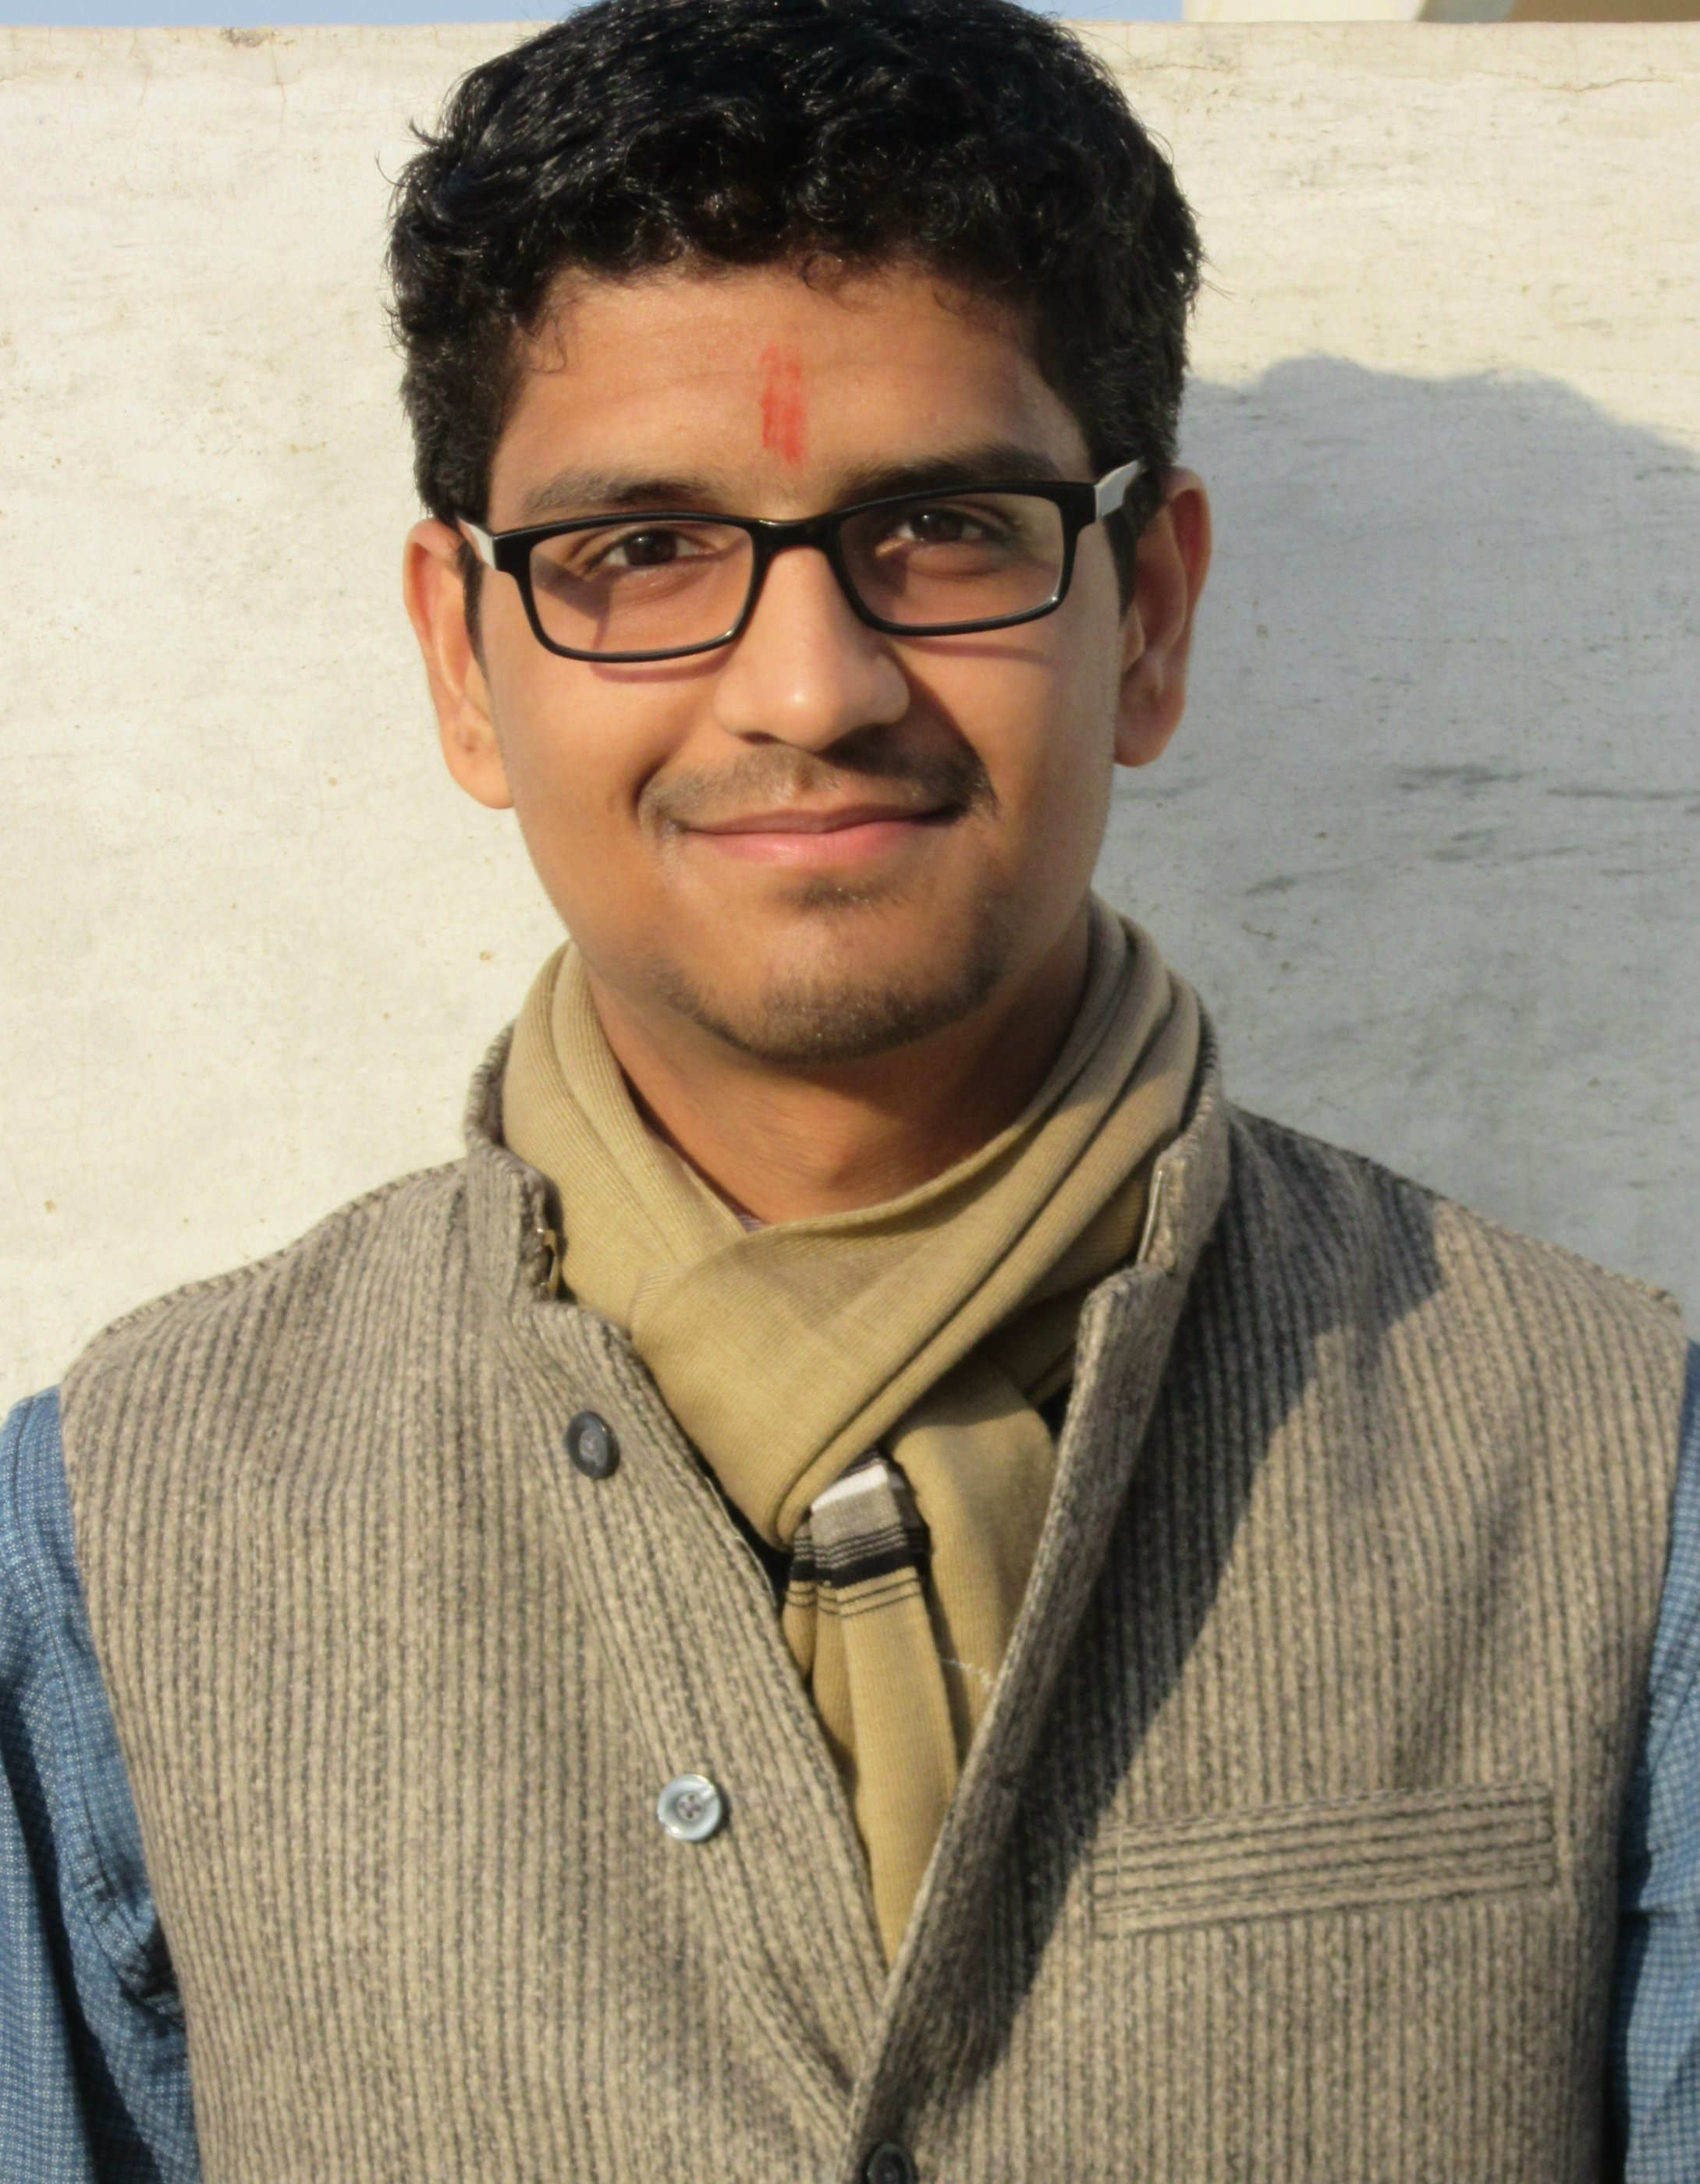
\includegraphics[width=90px]{Abhishek}
	\end{figure}
	
	%%%%%%%%%%%%%  OBJECTIVE   %%%%%%%%%%%
	\begin{flushleft}
		\textbf{OBJECTIVE}
		
		\vspace{-0.20in}
		\hspace{1.5in}
		To enhance my technical skills and implement it for mankind.\\
	\end{flushleft}
	
	%%%%%%%%%%%%   EDUCATION   %%%%%%%%%
	\begin{flushleft}
		
		\textbf{EDUCATION}
	\end{flushleft}
	
	\begin{tabular}{|c|c|c|c|c|}
		\hline
		\textbf{Certificate} & \textbf{School/College} & \textbf{Board/University} &  \textbf{year} & \textbf{Pass}   \\
		&        &            &              & \textbf{Percentage}\\
		\hline
		
		Secondary & Basic English Sr. & Board of Secondary Education & 2010-2011 &88.17 \\
		Examination&Sec. School,Bikaner & Rajasthan, Ajmer& & \\
		\hline
		Sr. Secondary & Basic English Sr. & Board of Secondary Education & 2012-2013 &82.68 \\
		Examination&Sec. School,Bikaner & Rajasthan, Ajmer& & \\
		\hline
		B.Tech & National Institute & National Institute of  & 2013-2017 &7.77 CGPA\\
		(E.E.E)	&of Technology &Technology Meghalaya, & &(Till five \\
		& Meghalaya &Shillong-793003& &Semester) \\
		\hline
	\end{tabular}
	
	\end{document}